\chapter{Конструкторская часть}

В данном разделе будут рассмотрены схемы вышеизложенных алгоритмов.

\section{Разработка алгоритмов}

На рисунке \ref{img:linear} представлена схема последовательного алгоритма обработки матриц.

\begin{figure}[H]
	\begin{center}
		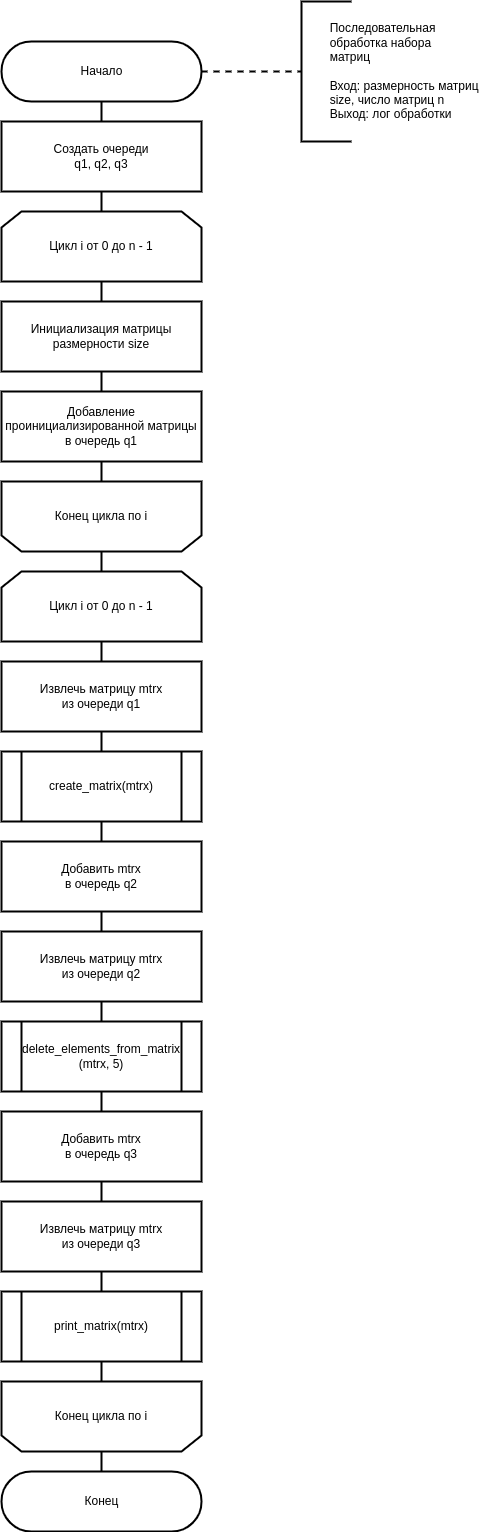
\includegraphics[scale=0.45]{img/linear.png}
	\end{center}
	\captionsetup{justification=centering}
	\caption{Последовательный алгоритм обработки матриц}
	\label{img:linear}
\end{figure}

На рисунке \ref{img:threads} представлена схема конвейерного алгоритма обработки матриц.

\begin{figure}[H]
	\begin{center}
		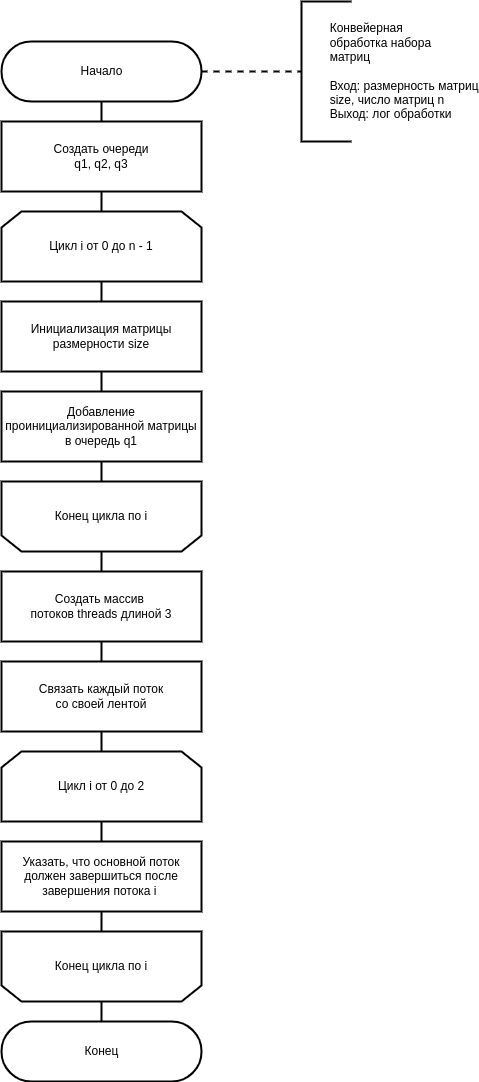
\includegraphics[scale=0.63]{img/threads.png}
	\end{center}
	\captionsetup{justification=centering}
	\caption{Конвейерный алгоритм обработки матриц}
	\label{img:threads}
\end{figure}

На рисунках \ref{img:first}--\ref{img:third} представлены схемы алгоритмов работы каждой ленты конвейера.

\begin{figure}[H]
	\begin{center}
		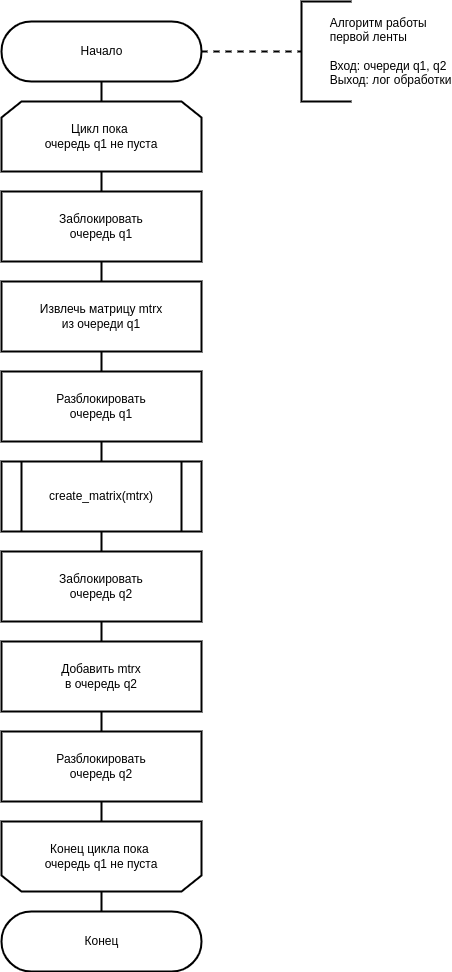
\includegraphics[scale=0.63]{img/first.png}
	\end{center}
	\captionsetup{justification=centering}
	\caption{Алгоритм работы первой ленты}
	\label{img:first}
\end{figure}

\begin{figure}[H]
	\begin{center}
		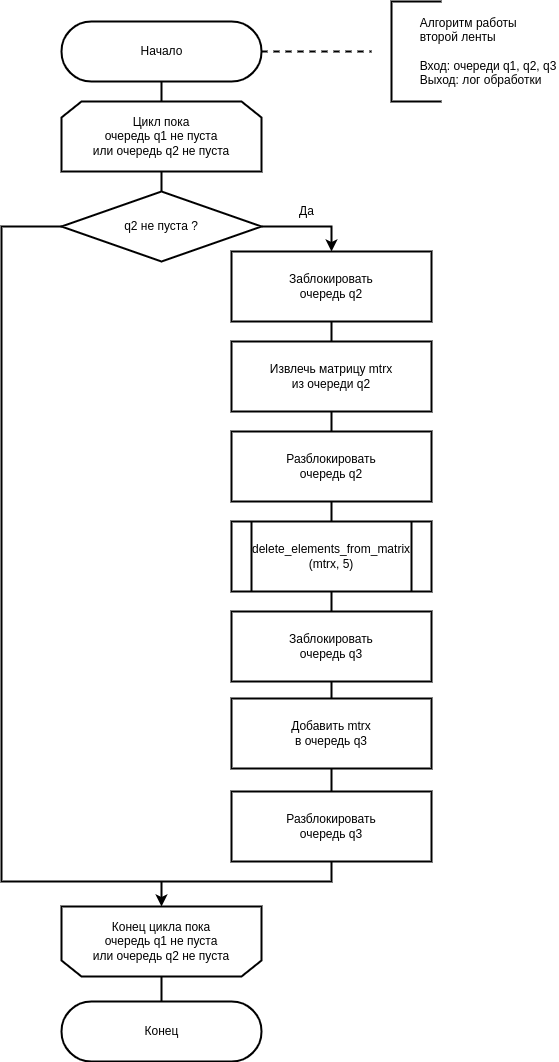
\includegraphics[scale=0.63]{img/second.png}
	\end{center}
	\captionsetup{justification=centering}
	\caption{Алгоритм работы второй ленты}
	\label{img:second}
\end{figure}


\begin{figure}[H]
	\begin{center}
		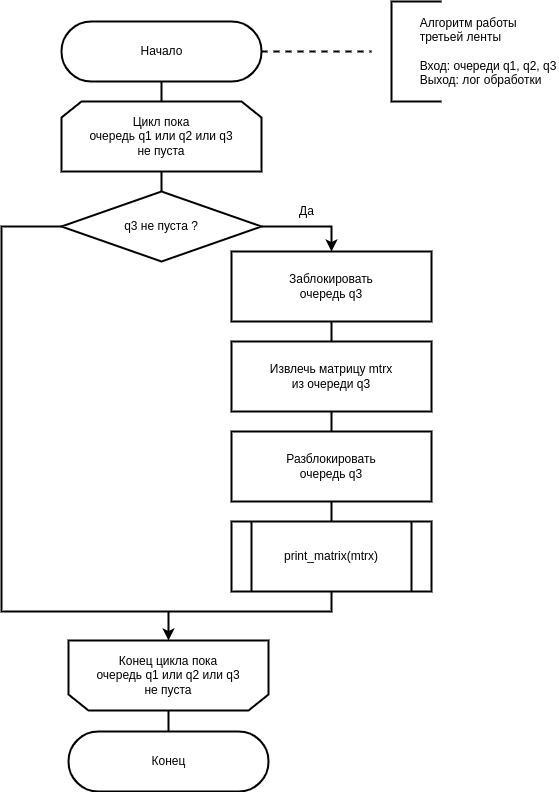
\includegraphics[scale=0.7]{img/third.png}
	\end{center}
	\captionsetup{justification=centering}
	\caption{Алгоритм работы третьей ленты}
	\label{img:third}
\end{figure}

На рисунке \ref{img:creation} представлена схема алгоритма генерации верхнетреугольной упакованной в КРМ-схему хранения матрицы.

\begin{figure}[H]
	\begin{center}
		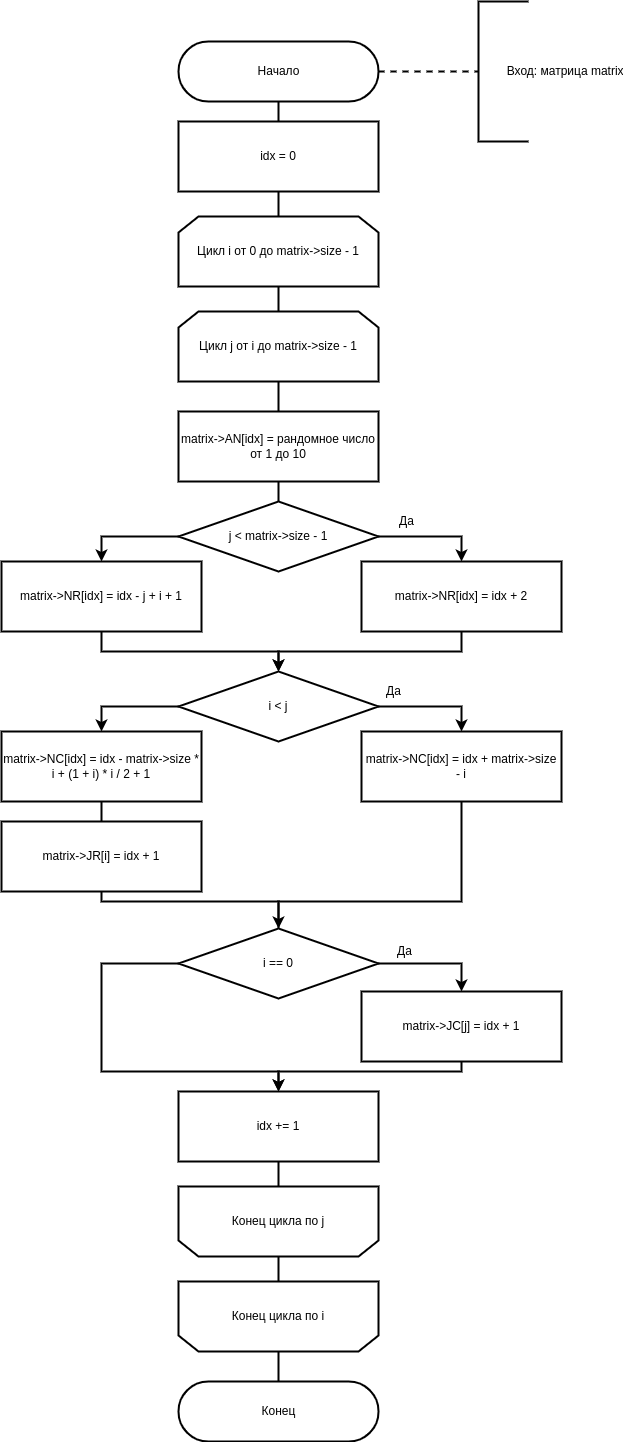
\includegraphics[scale=0.47]{img/creation.png}
	\end{center}
	\captionsetup{justification=centering}
	\caption{Схема алгоритма генерации матрицы}
	\label{img:creation}
\end{figure}

На рисунках \ref{img:deletion1}--\ref{img:deletion3} представлена схема алгоритма удаления из матрицы элементов, меньших или равных q.

\begin{figure}[H]
	\begin{center}
		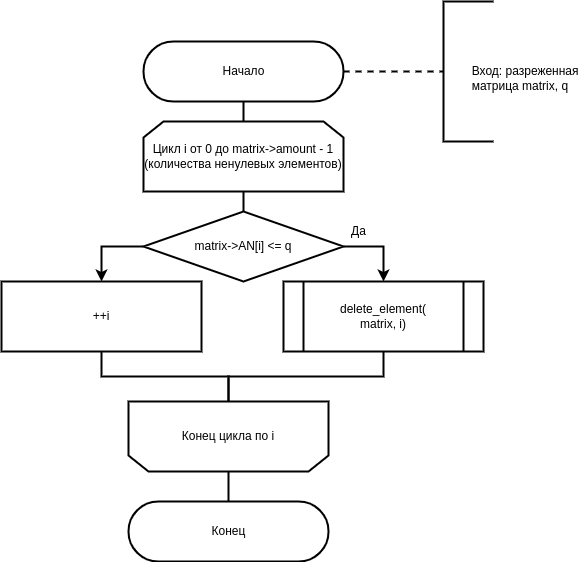
\includegraphics[scale=0.51]{img/deletion1.png}
	\end{center}
	\captionsetup{justification=centering}
	\caption{Схема алгоритма удаления элементов (1 часть)}
	\label{img:deletion1}
\end{figure}

\begin{figure}[H]
	\begin{center}
		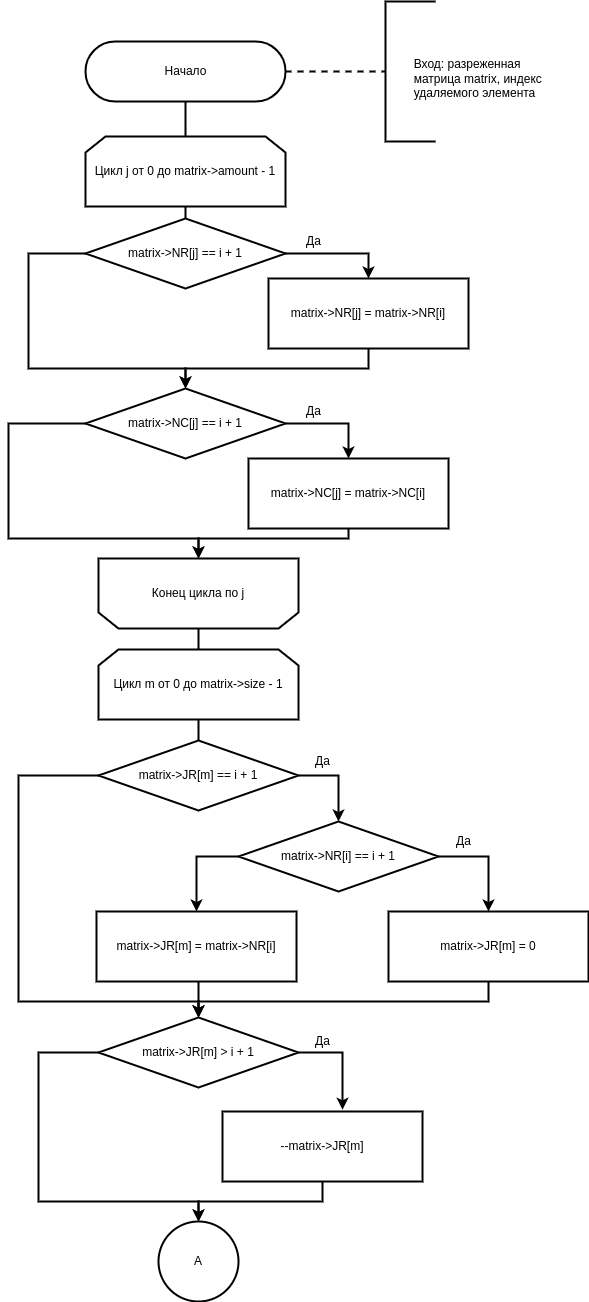
\includegraphics[scale=0.51]{img/deletion2.png}
	\end{center}
	\captionsetup{justification=centering}
	\caption{Схема алгоритма удаления элементов (2 часть)}
	\label{img:deletion2}
\end{figure}

\begin{figure}[H]
	\begin{center}
		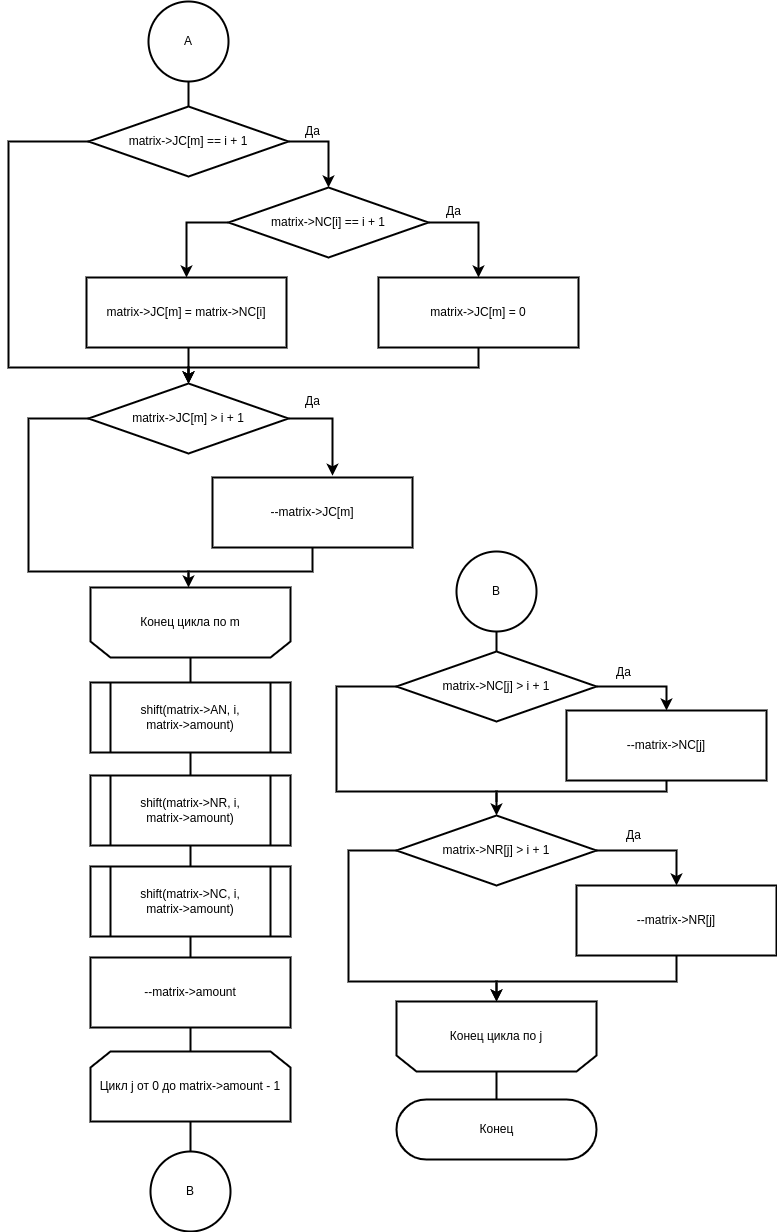
\includegraphics[scale=0.51]{img/deletion3.png}
	\end{center}
	\captionsetup{justification=centering}
	\caption{Схема алгоритма удаления элементов (3 часть)}
	\label{img:deletion3}
\end{figure}

На рисунке \ref{img:output} представлена схема алгоритма вывода матрицы в файл.

\begin{figure}[H]
	\begin{center}
		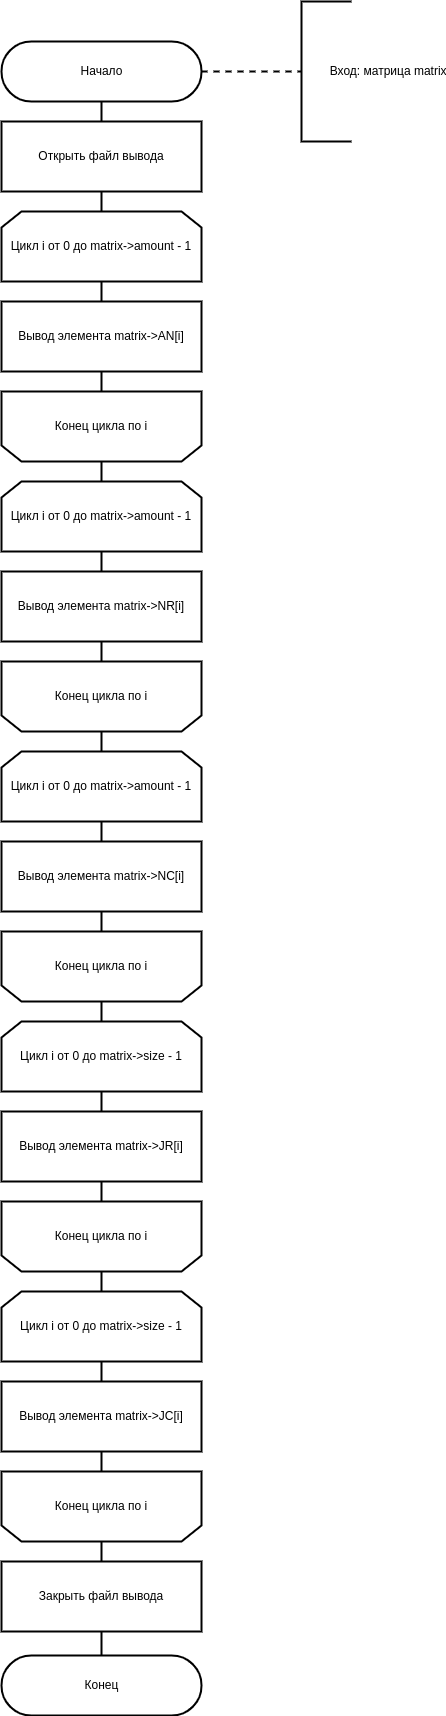
\includegraphics[scale=0.4]{img/output.png}
	\end{center}
	\captionsetup{justification=centering}
	\caption{Схема алгоритма вывода матрицы в файл}
	\label{img:output}
\end{figure}

\section*{Вывод}

На основе теоретических данных, полученных из аналитического раздела,
были построены схемы требуемых алгоритмов.
